\section{Experimental Evaluation}
\label{sec:eval}

In this section, LoRa protocol properties are discussed, and the presented implementations are evaluated through experiments.

\subsection{LoRa in Device-to-Device Scenarios}
LoRa as a long range protocol is limited in terms of bandwidth, since the resilient encoding scheme introduces some overhead and a duty cycle needs to be followed to fairly use the shared medium.
To understand the limitations of LoRa communication, some application-oriented examples are discussed.

\begin{figure}[ht!]
    \centering
    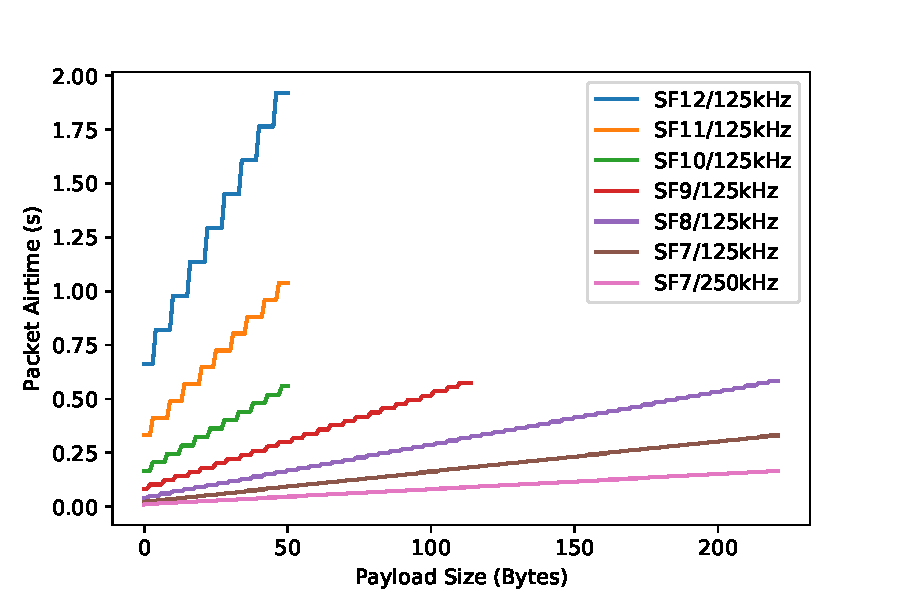
\includegraphics[width=.8\columnwidth]{gfx/lora-airtime.pdf}
    \caption{Exemplary packet airtime in different LoRa profiles.}
    \label{fig:lora-airtime}
\end{figure}

Figure~\ref{fig:lora-airtime} shows the payload sizes compared to the airtime required for sending with different spreading factors (SF), where the coding rate is set to 4/5.
The presented SF and channel bandwidth examples are taken from the EU standards (\cite{alliance2016lorawan}).
The message length of LoRa is limited depending on the SF to limit the airtime each individual message requires. 
The highest SFs are limited to a payload of 51 bytes. Using SF9, the payload can can go up to 115 bytes, and in the fastest SFs 8 and 7, messages can contain up to 222 bytes. 
SF12 packets, with the maximum payload of 51 bytes, take up to 1.92 seconds airtime, while 222 bytes in SF7/250 kHz only take 0.16 seconds.
When using LoRa for emergency communication, different profiles can be used to model, e.g., the importance of messages. 
Public service announcement of governmental institutions, including messages of rescuers can be sent in more resilient configurations, while chats of users helping each other in emergency situations can be limited to smaller areas, to cope with the limitations of the protocol.


\subsection{Device-To-Device Smartphone Communication}
We evaluated our proposed infrastructure-less LoRa communication via real world tests that cover two scenarios: (a) city area communication, and (b) rural area communication.

The motivation for scenario (a) are communication demands in disaster situations.
By having a low-cost companion device that extends the infrastructure-less communication range of our everyday devices could be a real benefit for such scenarios.
However, the inherent characteristics of cities, e.g., the high density of buildings, are a major problem for each wireless technology.

Scenario (b) is motivated by the fact that some rural areas, also in industrial countries, are still not covered by mobile networks (GSM, 3G, 4G, 5G).
The expectations of the tests in the rural areas therefore differ, since regions without obstacles might easily get good coverage, while areas with many trees might suffer from worse connections.

\subsubsection{Experimental Setup}

For the conducted tests, we used one fixed and one mobile station. 
The fixed station consists of a laptop logging the incoming messages. 
Figure~\ref{fig:evalsetup1} shows the mobile station, consisting of a smartphone in combination with a Heltec Wireless Stick driven by a Powerbank.
The default antenna was replaced by a +3dBi model, connected via SubMiniature version A (SMA).
The antennas of each station were 1.5 meter above the ground, in order to model realistic usage in device-to-device scenarios.

\begin{figure}[ht!]
    \centering
    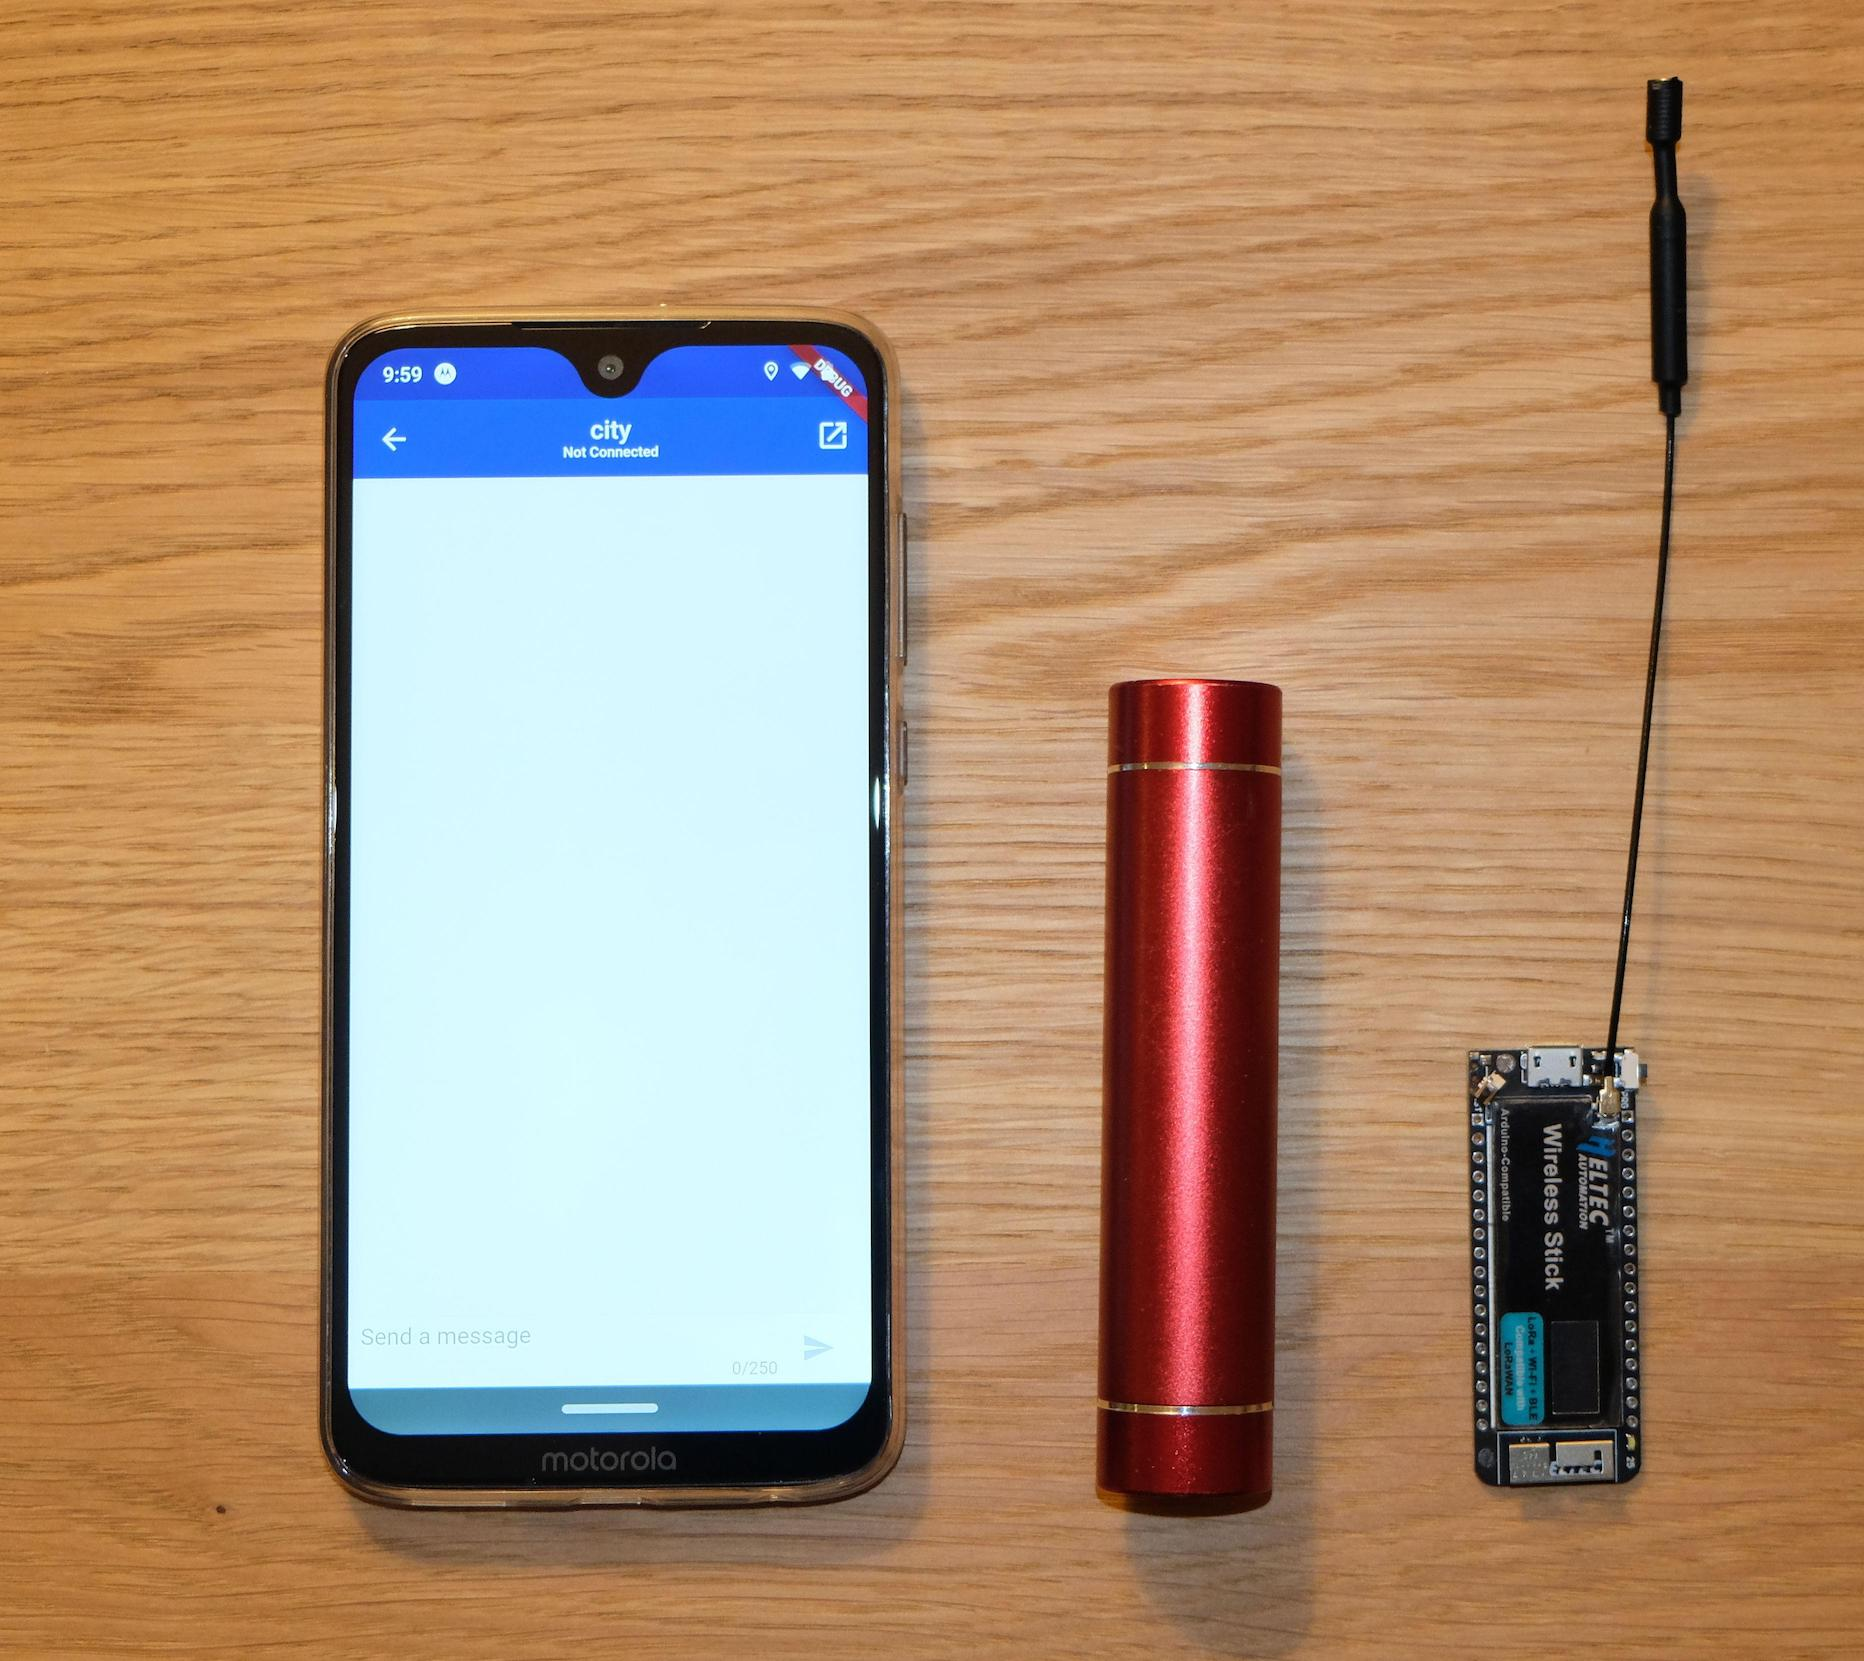
\includegraphics[width=.7\textwidth]{gfx/bluera-package.jpg}
    \caption{Mobile station: smartphone, power bank, and Heltec wireless stick.}
    \label{fig:evalsetup1}
\end{figure}

First, we selected one exemplary region for each of our two considered scenarios. 
The fixed station was then placed in the middle of the selected area and started listening for incoming messages.
For reproducibility and accuracy, we scripted message generation and sending on the mobile station, such that every 15 seconds one message including a GPS position was sent via Bluetooth LE and broadcasted by the companion device.
The mobile station was then moved away from the static station until no message could reach its counterpart anymore.
To observe a realistic model of device-to-device communication, the mobile station was moved in multiple directions.
The tests in both scenarios were repeated using two LoRa  profiles provided by \textit{rf95modem}: (a) Medium Range: Bandwidth: 125 kHz, Cr: 4/5, SF7, and (b) Long Range: Bandwidth: 125 kHz, Cr: 4/8, SF12.
Due to the simplicity of our test procedure, we did not get the maximum possible distances of our exemplary regions, but two real world setups, with distances that work even with the simple out-of-box experience of the rather low-cost Heltec wireless sticks.

\subsubsection{Results}

By analyzing the logs of the smartphone applications that transmit GPS locations of each sent message, we were able to calculate the distances of reliable communication setups between all participants for each scenario.

\begin{table}[ht!]
    \centering
    \begin{tabular}{llr}
        \toprule
        \textbf{Scenario}    & \textbf{Mode}          & \textbf{Maximum Distance} \\
        \midrule
        City        & (a) Medium Range  &  1.09 km \\
        & (b) Long Range    &  2.89 km \\
        Rural Area  & (a) Medium Range  &  1.31 km \\
        & (b) Long Range   &  1.64 km \\
        \bottomrule
    \end{tabular}
    \caption{Maximum distances achieved in the different areas and tested LoRa profiles in the conducted experiments.}
    \label{tab:max_dist}
\end{table}

Table~\ref{tab:max_dist} shows the maximum distances of the conducted tests.
For the Medium Range configuration, 1.09 km in the city area and 1.31 km in the rural area could be achieved.
With the rather high data rate of 5.47 kbps, the mode is a good choice in dense areas, where a larger amount of messages might occur, and airtime is limited.
In the Long Range profile, 1.64 km could be achieved in the rural area, while in the city scenario, some messages could be transmitted from 2.89 km range.

\begin{figure}[ht!]
    \centering
    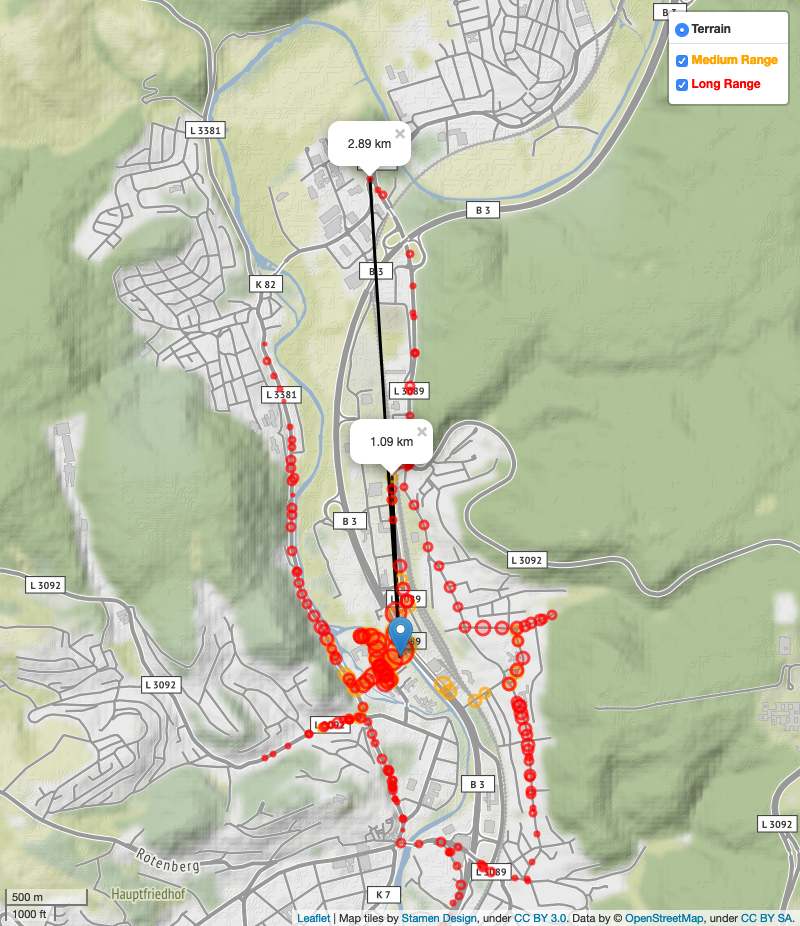
\includegraphics[width=\textwidth]{gfx/city.png}
    \caption{Successful LoRa transmissions in the city area.}
    \label{fig:eval_city_new}
\end{figure}

Figure~\ref{fig:eval_city_new} shows the results of the conducted tests in the city area.
The orange dots denote the Medium Range profile, while the red dots show the successful transmissions in the Long Range profile.
In the size of the markers, the Received Signal Strength Indicator (RSSI) is visualized. The larger the marker, the better the RSSI is. 
Note that in LoRa a higher SF enables a higher chance of successful decoding under worse RSSI values.
In the presented results, it is evident that LoRa works well as long as no obstacles are in the way. 
The maximum distance in the city area was achieved in the valley going through the city. 
Even though obstacles, such as buildings, were in the way, the signal could reach the other peer well.
When moving behind a hill, such as in the western or eastern parts of the presented map, the signal was not able to penetrate the obstacle.

\begin{figure}[ht!]
    \centering
    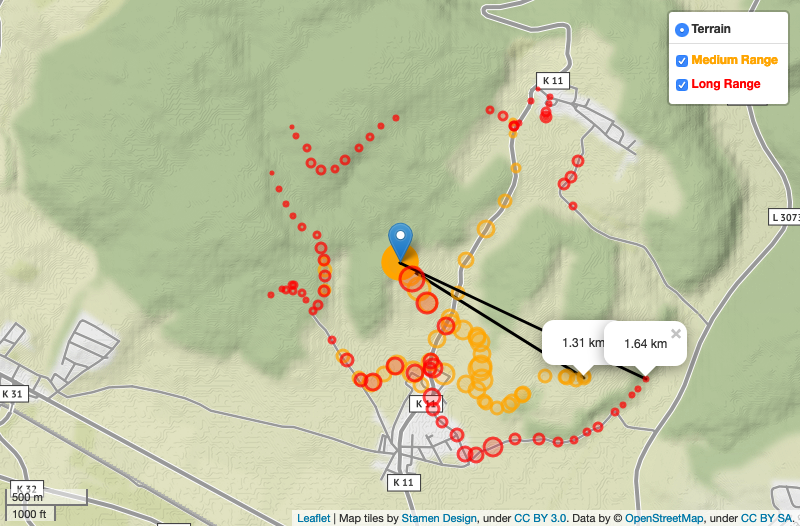
\includegraphics[width=\textwidth]{gfx/rural.png}
    \caption{Geo-positions of successful LoRa transmissions in a rural area.}
    \label{fig:eval_rural_new}
\end{figure}

In Figure~\ref{fig:eval_rural_new}, the successful LoRa transmission of the rural area are presented.
As excepted, the transmission range in the forested area is worse compared to the unforested area.
In the presented example, the northern part of the map consists of a forested area, while the southern part is mostly not forested.
From the plot, it can be observed that in the non-forested valley area, RSSI is high, and all LoRa messages are successfully transmitted in both modes. 
When forested areas and hills are in the line of sight, the RSSI worsens and quickly becomes unavailable.
In Long Range mode, transmission in forested places improves and messages are successfully transmitted through up to 600 meters of forested area.

\begin{figure}[ht!]
    \centering
    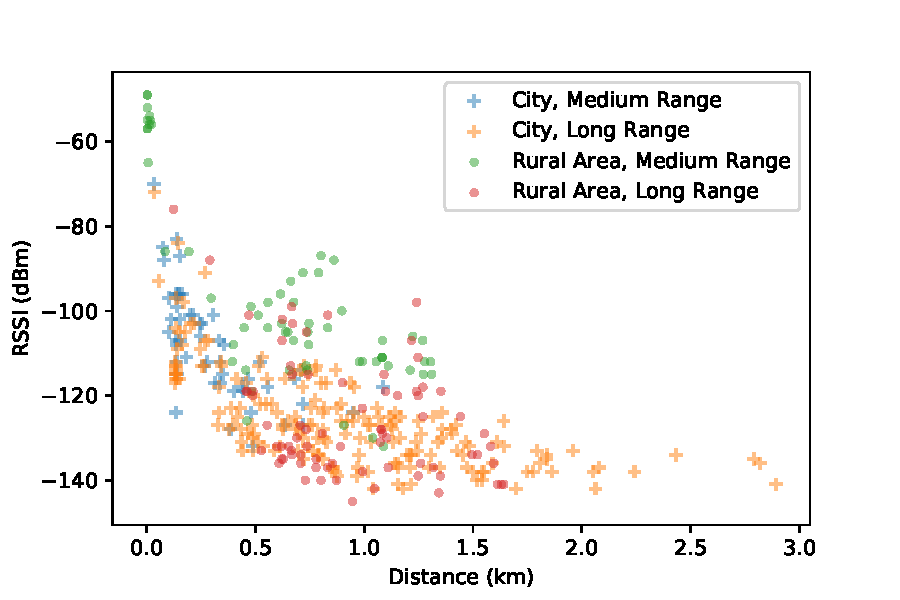
\includegraphics[width=.8\textwidth]{gfx/rssi-distance.pdf}
    \caption{Received Signal Strength Indicator in relation to transmission distance in the proposed device-to-device scenario.}
    \label{fig:eval_rssi}
\end{figure}

In Figure~\ref{fig:eval_rssi}, the observed RSSI values in relation to the distances are presented.
With the Long Range profile, signals with RSSI values of up to -140 dBm can be decoded successfully, while in the Medium Range profile the limit is around -130 dBm.

In general, this shows that LoRa is a viable option to enable device-to-device communication in crisis scenarios, where infrastructure is destroyed or temporarily not available.
The different profiles of LoRa can be used to limit communication to a certain area and therefore allow higher data rates, or cover a larger area and therefore reach out to more people. 


\subsection{Interfacing Emergency Networks}
When transmitting data over a disruption-tolerant network, an overhead is generated.
This is caused by the additional meta-data that a DTN bundle carries, e.g., the sender, receiver, or other blocks of information.
In addition, there is now a second overhead for the fragmentation header of the BBC.
Due to the small size of a LoRa packet, it is advisable to examine the total size of a transmission and the number of fragments.
The benefits or costs of the \texttt{xz} compression should also be considered.

For our evaluation, we created two types of payload data: randomly distributed data and the \emph{lorem ipsum} placeholder text.
The respective payloads were generated in the sizes of the power of two, from $2^1$ to $2^{11}$.
For this purpose, the 445 byte long lorem ipsum text was shortened or repeated accordingly.
This payload was wrapped into a DTN packet, sent from \texttt{dtn://source/} to \texttt{dtn://destination/} with an additional age block to set the lifetime to one hour.
The LoRa maximum payload can be up to 251 bytes in size, as instructed by \textit{rf95modem} in our test configuration.

\begin{figure}[ht!]
    \centering
    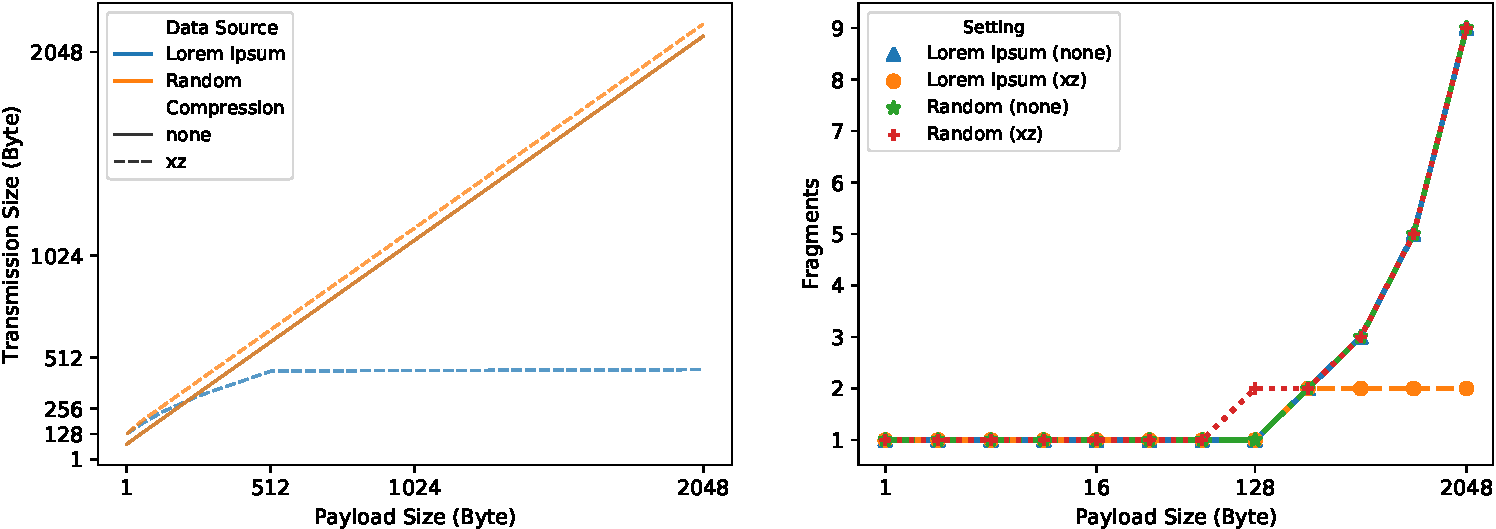
\includegraphics[width=\columnwidth]{gfx/dtn7-bbc-eval.pdf}
    \caption{Total transmission size and amount of fragments for different payloads.}
    \label{fig:dtn7_bbc_eval}
\end{figure}

The overhead of a DTN bundle is 77 bytes without compression.
In Figure~\ref{fig:dtn7_bbc_eval}, the final transmission size and the number of required fragments are shown for the two characteristics of the payload data and its size.
It is noticeable that for a random payload the transmission size is slightly larger.
However, the number of fragments is almost always the same.
Furthermore, user data is usually not randomly distributed.
This is where the advantage of the compression comes into effect, as it becomes evident especially in the low number of fragments with compressed payloads.

We also carried out a small field test.
For this purpose, three DTN nodes were installed, each equipped with a \textit{rf95modem} for 868 MHz in the Short Range profile: 500 kHz, Cr: 4/5, SF7.
The nodes were positioned so that only one node had direct radio contact with the other two.
Every time a packet is forwarded in a DTN, some meta-data is updated, e.g., the Previous Node to specify the last relaying node.
To verify the packet forwarding, we inspected the Previous Node from the received packet.
If this value does not match the packet's sender, it was successfully forwarded.
To perform this evaluation, we prepared three nodes, $n_0$, $n_1$, and $n_2$.
$n_1$ was positioned in the midpoint, further $n_0$ and $n_2$ were not supposed to have direct contact.
Outgoing from $n_0$, packets were sent addressed to $n_2$.
These should be transferred from $n_0$ to $n_1$ first and forwarded from $n_1$ to $n_2$ afterwards.
We then sent DTN packets with a small payload so that they fit into a single LoRa packet.
As a result, we observed situations where the Previous Node was adjusted accordingly.
In such a case, the round trip time took 1.7 seconds from initiating the transmission to receiving the acknowledgement of reception.


\subsection{Energy Considerations}
While the energy consumption of smartphones is a well studied field and battery lifetimes of these devices are up to some days, the companion devices studied in this paper are not evaluated that well.
Thus, we measured multiple devices targeted by the proposed firmware in terms of energy usage in different energy states, namely receiving, sending, and deep sleep.
From these measurements, the required battery capacities can be inferred.
%
\begin{table}[ht!]
    \centering
    \footnotesize
    \begin{tabularx}{\textwidth}{Xlllll}
        \toprule
        \textbf{Board}             & \textbf{Receiving} & \textbf{Sending} & \textbf{Deep Sleep} & \textbf{Additional Features} & \textbf{Price} \\
        \midrule
        TTGO T-Fox 27 dB           & 392 mW          & 1,771 mW      & 61 mW            & WiFi, BLE, OLED, RTC & ~20 €         \\
        TTGO T-Fox 20 dB           & 400 mW          & 902 mW        & 61 mW            & WiFi, BLE, OLED, RTC & ~20 €         \\
        TTGO LORA ESP32            & 404 mW          & 782 mW        & 68 mW            & WiFi, BLE & ~15 €                   \\
        TTGO LORA32 V2.0           & 393 mW          & 689 mW        & 57 mW            & WiFi, BLE, OLED, SD & ~20 €         \\
        TTGO LORA32 V2.1\_1.6      & 387 mW          & 785 mW        & 57 mW            & WiFi, BLE, OLED, SD & ~20  €          \\
        Heltec Wireless Stick      & 391 mW          & 923 mW        & 76 mW            & WiFi, BLE, OLED  & ~12  €            \\
        Adafruit Feather 32u4 LoRa & 72 mW           & 648 mW        & 49 mW            & -   & ~35  €                           \\
        Adafruit Feather M0 LoRa   & 95 mW           & 697 mW        & \textless 1 mW   & -    & ~35  €                          \\
        TTGO T-Beam v0.7           & 723 mW          & 1,125 mW      & 393 mW           & WiFi, BLE, GPS  & ~20  €             \\
        \bottomrule
\end{tabularx}
\caption{Energy consumption in receiving, sending, and deep sleep modes of \textit{rf95modem} compatible boards.}
\label{tab:energy}
\end{table}
%

The energy consumption was measured using an ODROID Smart Power Meter\footnote{\url{https://www.hardkernel.com/shop/smart-power/}} connected to the microUSB connector of the board and supplied 5 V.

In Table~\ref{tab:energy}, the average energy consumption of the listed boards is presented. 
Since the boards need to be online to receive messages from other boards, the receiving mode has the highest impact on energy consumption.

The power consumption of the measured boards when receiving data shows a broad variance, e.g., from about 72 mW for the Adafruit Feather 32u4 LoRa board up to 723 mW for the TTGO T-Beam v0.7 board.
While sending data, the required power differences become more balanced.
When deployed in sensor networks, the deep sleep power consumption becomes important. 
Four of the tested boards require 49 to 76 mW in this mode, while one board requires below 1 mW.
The values for deep sleep are likely caused by powering the boards through the microUSB connection, which requires a transformation to the voltage required by the microprocessors. 
Also, most boards contain a serial to USB converter, which cannot be turned off when powered via USB.

To put these numbers into perspective, we assume a powerbank with a capacity of up to 20,000 mAh. Such powerbanks are widespread and used by smartphone users to recharge their phones. 
This capacity at 3.3 volts relates to 66 Wh, and thus can power the TTGO and Heltec hardware for more than 160 hours. 
The maximum receiving time can be achieved using the Feather 32u4 LoRa board with more than 900 hours of receiving time.
